\documentclass[twoside]{book}

% Packages required by doxygen
\usepackage{fixltx2e}
\usepackage{calc}
\usepackage{doxygen}
\usepackage[export]{adjustbox} % also loads graphicx
\usepackage{graphicx}
\usepackage[utf8]{inputenc}
\usepackage{makeidx}
\usepackage{multicol}
\usepackage{multirow}
\PassOptionsToPackage{warn}{textcomp}
\usepackage{textcomp}
\usepackage[nointegrals]{wasysym}
\usepackage[table]{xcolor}

% Font selection
\usepackage[T1]{fontenc}
\usepackage[scaled=.90]{helvet}
\usepackage{courier}
\usepackage{amssymb}
\usepackage{sectsty}
\renewcommand{\familydefault}{\sfdefault}
\allsectionsfont{%
  \fontseries{bc}\selectfont%
  \color{darkgray}%
}
\renewcommand{\DoxyLabelFont}{%
  \fontseries{bc}\selectfont%
  \color{darkgray}%
}
\newcommand{\+}{\discretionary{\mbox{\scriptsize$\hookleftarrow$}}{}{}}

% Page & text layout
\usepackage{geometry}
\geometry{%
  a4paper,%
  top=2.5cm,%
  bottom=2.5cm,%
  left=2.5cm,%
  right=2.5cm%
}
\tolerance=750
\hfuzz=15pt
\hbadness=750
\setlength{\emergencystretch}{15pt}
\setlength{\parindent}{0cm}
\setlength{\parskip}{3ex plus 2ex minus 2ex}
\makeatletter
\renewcommand{\paragraph}{%
  \@startsection{paragraph}{4}{0ex}{-1.0ex}{1.0ex}{%
    \normalfont\normalsize\bfseries\SS@parafont%
  }%
}
\renewcommand{\subparagraph}{%
  \@startsection{subparagraph}{5}{0ex}{-1.0ex}{1.0ex}{%
    \normalfont\normalsize\bfseries\SS@subparafont%
  }%
}
\makeatother

% Headers & footers
\usepackage{fancyhdr}
\pagestyle{fancyplain}
\fancyhead[LE]{\fancyplain{}{\bfseries\thepage}}
\fancyhead[CE]{\fancyplain{}{}}
\fancyhead[RE]{\fancyplain{}{\bfseries\leftmark}}
\fancyhead[LO]{\fancyplain{}{\bfseries\rightmark}}
\fancyhead[CO]{\fancyplain{}{}}
\fancyhead[RO]{\fancyplain{}{\bfseries\thepage}}
\fancyfoot[LE]{\fancyplain{}{}}
\fancyfoot[CE]{\fancyplain{}{}}
\fancyfoot[RE]{\fancyplain{}{\bfseries\scriptsize Generated by Doxygen }}
\fancyfoot[LO]{\fancyplain{}{\bfseries\scriptsize Generated by Doxygen }}
\fancyfoot[CO]{\fancyplain{}{}}
\fancyfoot[RO]{\fancyplain{}{}}
\renewcommand{\footrulewidth}{0.4pt}
\renewcommand{\chaptermark}[1]{%
  \markboth{#1}{}%
}
\renewcommand{\sectionmark}[1]{%
  \markright{\thesection\ #1}%
}

% Indices & bibliography
\usepackage{natbib}
\usepackage[titles]{tocloft}
\setcounter{tocdepth}{3}
\setcounter{secnumdepth}{5}
\makeindex

% Hyperlinks (required, but should be loaded last)
\usepackage{ifpdf}
\ifpdf
  \usepackage[pdftex,pagebackref=true]{hyperref}
\else
  \usepackage[ps2pdf,pagebackref=true]{hyperref}
\fi
\hypersetup{%
  colorlinks=true,%
  linkcolor=blue,%
  citecolor=blue,%
  unicode%
}

% Custom commands
\newcommand{\clearemptydoublepage}{%
  \newpage{\pagestyle{empty}\cleardoublepage}%
}

\usepackage{caption}
\captionsetup{labelsep=space,justification=centering,font={bf},singlelinecheck=off,skip=4pt,position=top}

%===== C O N T E N T S =====

\begin{document}

% Titlepage & ToC
\hypersetup{pageanchor=false,
             bookmarksnumbered=true,
             pdfencoding=unicode
            }
\pagenumbering{alph}
\begin{titlepage}
\vspace*{7cm}
\begin{center}%
{\Large unhangman }\\
\vspace*{1cm}
{\large Generated by Doxygen 1.8.13}\\
\end{center}
\end{titlepage}
\clearemptydoublepage
\pagenumbering{roman}
\tableofcontents
\clearemptydoublepage
\pagenumbering{arabic}
\hypersetup{pageanchor=true}

%--- Begin generated contents ---
\chapter{Welcome to unhangman}
\label{index}\hypertarget{index}{}\hypertarget{index_intro_sec}{}\section{Introduction}\label{index_intro_sec}
This is a collection of functions designed to help you build a crossword / hangman game / solver.\hypertarget{index_usage}{}\section{Usage}\label{index_usage}
See the \hyperlink{unhangman_8h}{include/unhangman.\+h} in the files tab. 
\chapter{File Index}
\section{File List}
Here is a list of all documented files with brief descriptions\+:\begin{DoxyCompactList}
\item\contentsline{section}{include/\hyperlink{unhangman_8h}{unhangman.\+h} \\*Declarations of all the functions }{\pageref{unhangman_8h}}{}
\item\contentsline{section}{src/\hyperlink{unhangman_8cpp}{unhangman.\+cpp} \\*Implementations of all the functions }{\pageref{unhangman_8cpp}}{}
\end{DoxyCompactList}

\chapter{File Documentation}
\hypertarget{unhangman_8h}{}\section{include/unhangman.h File Reference}
\label{unhangman_8h}\index{include/unhangman.\+h@{include/unhangman.\+h}}


Declarations of all the functions.  


{\ttfamily \#include $<$string$>$}\newline
{\ttfamily \#include $<$vector$>$}\newline
{\ttfamily \#include $<$map$>$}\newline
{\ttfamily \#include $<$experimental/optional$>$}\newline
Include dependency graph for unhangman.\+h\+:\nopagebreak
\begin{figure}[H]
\begin{center}
\leavevmode
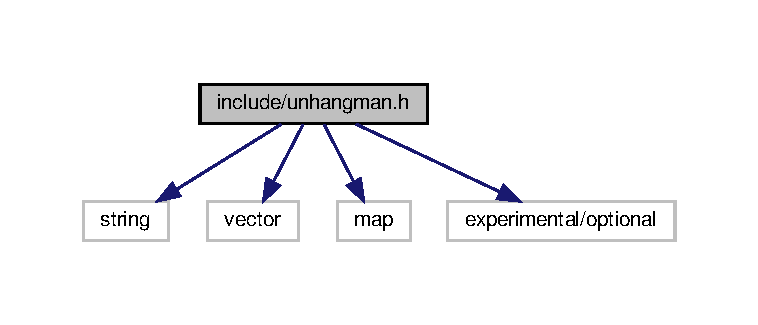
\includegraphics[width=350pt]{unhangman_8h__incl}
\end{center}
\end{figure}
This graph shows which files directly or indirectly include this file\+:\nopagebreak
\begin{figure}[H]
\begin{center}
\leavevmode
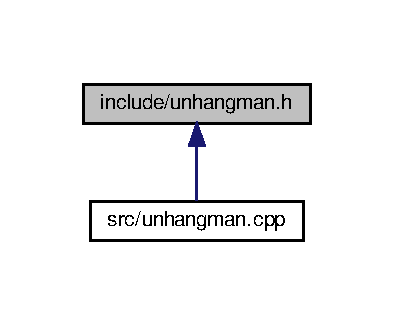
\includegraphics[width=189pt]{unhangman_8h__dep__incl}
\end{center}
\end{figure}
\subsection*{Functions}
\begin{DoxyCompactItemize}
\item 
std\+::vector$<$ std\+::string $>$ \hyperlink{unhangman_8h_ada47e9338f9e87b423f8214dc4a736e6}{read\+\_\+dictionary} (const std\+::string \&path)
\begin{DoxyCompactList}\small\item\em Fill a vector of strings from a file. \end{DoxyCompactList}\item 
std\+::vector$<$ std\+::string $>$ \hyperlink{unhangman_8h_a4905d4615c76e8b03b2485034f1dbda1}{filter\+\_\+length} (const std\+::vector$<$ std\+::string $>$ \&dictionary, unsigned length)
\begin{DoxyCompactList}\small\item\em Filters out words that don\textquotesingle{}t match the desired length. \end{DoxyCompactList}\item 
std\+::vector$<$ std\+::string $>$ \hyperlink{unhangman_8h_a99534dccde214cf085d0e571a09d6cc5}{filter\+\_\+pattern} (const std\+::vector$<$ std\+::string $>$ \&dictionary, const std\+::string \&pattern, char wildcard=\textquotesingle{} $\ast$\textquotesingle{})
\begin{DoxyCompactList}\small\item\em Filter words that dont match the provided pattern. \end{DoxyCompactList}\item 
std\+::map$<$ char, unsigned $>$ \hyperlink{unhangman_8h_a1622b1d311b2495ae299f8c875a5573d}{count\+\_\+character\+\_\+frequency} (const std\+::vector$<$ std\+::string $>$ \&dictionary, const std\+::string \&pattern=\char`\"{}\char`\"{})
\begin{DoxyCompactList}\small\item\em Counts the appearance of characters in words. Each character is counted once per word. If it\textquotesingle{}s possition matches the pattern\textquotesingle{}s, it\textquotesingle{}s ignored. \end{DoxyCompactList}\item 
std\+::vector$<$ char $>$ \hyperlink{unhangman_8h_a3663781c1785f8bd725da940b07e2fb9}{frequency\+\_\+to\+\_\+array} (const std\+::map$<$ char, unsigned $>$ \&character\+\_\+frequency)
\begin{DoxyCompactList}\small\item\em Transforms a map of characters and their appearance counters to an array sorted by the appearance counter. \end{DoxyCompactList}\item 
std\+::experimental\+::optional$<$ char $>$ \hyperlink{unhangman_8h_ac09e771692a2604aa55d5675a3802fd2}{get\+\_\+next\+\_\+char} (const std\+::vector$<$ char $>$ \&char\+\_\+array, const std\+::string \&ignore=\char`\"{}\char`\"{})
\begin{DoxyCompactList}\small\item\em Get the character that apeared in the most words. \end{DoxyCompactList}\item 
std\+::experimental\+::optional$<$ char $>$ \hyperlink{unhangman_8h_a75083dc0d9702a9641461d8a4c14bbca}{get\+\_\+next\+\_\+vowel} (const std\+::vector$<$ char $>$ \&char\+\_\+array, const std\+::string \&ignore=\char`\"{}\char`\"{})
\begin{DoxyCompactList}\small\item\em Get the vowel that apeared in the most words. \end{DoxyCompactList}\item 
std\+::experimental\+::optional$<$ char $>$ \hyperlink{unhangman_8h_a223617d2b5703642d65670e7f49d2a5e}{get\+\_\+next\+\_\+constant} (const std\+::vector$<$ char $>$ \&char\+\_\+array, const std\+::string \&ignore=\char`\"{}\char`\"{})
\begin{DoxyCompactList}\small\item\em Get the constatnt that apeared in the most words. \end{DoxyCompactList}\item 
std\+::experimental\+::optional$<$ std\+::vector$<$ unsigned $>$ $>$ \hyperlink{unhangman_8h_a8b79ef16e04c4f46d2204a618a3b6fb9}{find\+\_\+char\+\_\+positions} (const std\+::vector$<$ std\+::string $>$ \&dictionary, char c)
\begin{DoxyCompactList}\small\item\em If a character appears in the same possitions in all provided words, it returns their positions. \end{DoxyCompactList}\item 
std\+::string \hyperlink{unhangman_8h_ab1474fd24375a98e650b739becf090a3}{remove\+\_\+pattern} (const std\+::string \&word, const std\+::string \&pattern, char wildcard=\textquotesingle{} $\ast$\textquotesingle{})
\begin{DoxyCompactList}\small\item\em Removes the characters of pattern from word. \end{DoxyCompactList}\item 
std\+::vector$<$ std\+::string $>$ \hyperlink{unhangman_8h_a57fca433ea4c6ee0693e612668c383e4}{must\+\_\+contain} (const std\+::vector$<$ std\+::string $>$ \&dictionary, char c, const std\+::string \&pattern=\char`\"{}\char`\"{})
\begin{DoxyCompactList}\small\item\em Returns a vector of words that contain the specified character, ignoring it\textquotesingle{}s appearence in the pattern (if provided) \end{DoxyCompactList}\item 
std\+::vector$<$ std\+::string $>$ \hyperlink{unhangman_8h_aa0d9948dada05cb5694dae370b69fc0b}{must\+\_\+not\+\_\+contain} (const std\+::vector$<$ std\+::string $>$ \&dictionary, char c, const std\+::string \&pattern=\char`\"{}\char`\"{})
\begin{DoxyCompactList}\small\item\em Returns a vector of words that don\textquotesingle{}t contain the specified character, ignoring it\textquotesingle{}s appearence in the pattern (if provided) \end{DoxyCompactList}\end{DoxyCompactItemize}


\subsection{Detailed Description}
Declarations of all the functions. 



\subsection{Function Documentation}
\mbox{\Hypertarget{unhangman_8h_a1622b1d311b2495ae299f8c875a5573d}\label{unhangman_8h_a1622b1d311b2495ae299f8c875a5573d}} 
\index{unhangman.\+h@{unhangman.\+h}!count\+\_\+character\+\_\+frequency@{count\+\_\+character\+\_\+frequency}}
\index{count\+\_\+character\+\_\+frequency@{count\+\_\+character\+\_\+frequency}!unhangman.\+h@{unhangman.\+h}}
\subsubsection{\texorpdfstring{count\+\_\+character\+\_\+frequency()}{count\_character\_frequency()}}
{\footnotesize\ttfamily std\+::map$<$char, unsigned$>$ count\+\_\+character\+\_\+frequency (\begin{DoxyParamCaption}\item[{const std\+::vector$<$ std\+::string $>$ \&}]{dictionary,  }\item[{const std\+::string \&}]{pattern = {\ttfamily \char`\"{}\char`\"{}} }\end{DoxyParamCaption})}



Counts the appearance of characters in words. Each character is counted once per word. If it\textquotesingle{}s possition matches the pattern\textquotesingle{}s, it\textquotesingle{}s ignored. 


\begin{DoxyParams}{Parameters}
{\em dictionary} & The words to check \\
\hline
{\em pattern} & The pattern to ignore\\
\hline
\end{DoxyParams}
\begin{DoxyReturn}{Returns}
A map of characters and their appearance counters 
\end{DoxyReturn}
\mbox{\Hypertarget{unhangman_8h_a4905d4615c76e8b03b2485034f1dbda1}\label{unhangman_8h_a4905d4615c76e8b03b2485034f1dbda1}} 
\index{unhangman.\+h@{unhangman.\+h}!filter\+\_\+length@{filter\+\_\+length}}
\index{filter\+\_\+length@{filter\+\_\+length}!unhangman.\+h@{unhangman.\+h}}
\subsubsection{\texorpdfstring{filter\+\_\+length()}{filter\_length()}}
{\footnotesize\ttfamily std\+::vector$<$std\+::string$>$ filter\+\_\+length (\begin{DoxyParamCaption}\item[{const std\+::vector$<$ std\+::string $>$ \&}]{dictionary,  }\item[{unsigned}]{length }\end{DoxyParamCaption})}



Filters out words that don\textquotesingle{}t match the desired length. 


\begin{DoxyParams}{Parameters}
{\em dictionary} & The words to check \\
\hline
{\em length} & The required length\\
\hline
\end{DoxyParams}
\begin{DoxyReturn}{Returns}
A vector$<$string$>$ of words that match the length 
\end{DoxyReturn}
\mbox{\Hypertarget{unhangman_8h_a99534dccde214cf085d0e571a09d6cc5}\label{unhangman_8h_a99534dccde214cf085d0e571a09d6cc5}} 
\index{unhangman.\+h@{unhangman.\+h}!filter\+\_\+pattern@{filter\+\_\+pattern}}
\index{filter\+\_\+pattern@{filter\+\_\+pattern}!unhangman.\+h@{unhangman.\+h}}
\subsubsection{\texorpdfstring{filter\+\_\+pattern()}{filter\_pattern()}}
{\footnotesize\ttfamily std\+::vector$<$std\+::string$>$ filter\+\_\+pattern (\begin{DoxyParamCaption}\item[{const std\+::vector$<$ std\+::string $>$ \&}]{dictionary,  }\item[{const std\+::string \&}]{pattern,  }\item[{char}]{wildcard = {\ttfamily \textquotesingle{}~$\ast$\textquotesingle{}} }\end{DoxyParamCaption})}



Filter words that dont match the provided pattern. 


\begin{DoxyParams}{Parameters}
{\em dictionary} & The words to check \\
\hline
{\em pattern} & A string to match all words. E.\+g. \char`\"{}pot$\ast$to\char`\"{} \\
\hline
{\em wildcard} & The character to ignore in the pattern. Default \textquotesingle{}$\ast$\textquotesingle{}\\
\hline
\end{DoxyParams}
\begin{DoxyReturn}{Returns}
A vector$<$string$>$ of words that match the pattern 
\end{DoxyReturn}
\mbox{\Hypertarget{unhangman_8h_a8b79ef16e04c4f46d2204a618a3b6fb9}\label{unhangman_8h_a8b79ef16e04c4f46d2204a618a3b6fb9}} 
\index{unhangman.\+h@{unhangman.\+h}!find\+\_\+char\+\_\+positions@{find\+\_\+char\+\_\+positions}}
\index{find\+\_\+char\+\_\+positions@{find\+\_\+char\+\_\+positions}!unhangman.\+h@{unhangman.\+h}}
\subsubsection{\texorpdfstring{find\+\_\+char\+\_\+positions()}{find\_char\_positions()}}
{\footnotesize\ttfamily std\+::experimental\+::optional$<$std\+::vector$<$unsigned$>$ $>$ find\+\_\+char\+\_\+positions (\begin{DoxyParamCaption}\item[{const std\+::vector$<$ std\+::string $>$ \&}]{dictionary,  }\item[{char}]{c }\end{DoxyParamCaption})}



If a character appears in the same possitions in all provided words, it returns their positions. 


\begin{DoxyParams}{Parameters}
{\em dictionary} & The words to check \\
\hline
{\em c} & The character to find positions\\
\hline
\end{DoxyParams}
\begin{DoxyReturn}{Returns}
A vector$<$unsigned$>$ with the positions of the character 
\end{DoxyReturn}
\mbox{\Hypertarget{unhangman_8h_a3663781c1785f8bd725da940b07e2fb9}\label{unhangman_8h_a3663781c1785f8bd725da940b07e2fb9}} 
\index{unhangman.\+h@{unhangman.\+h}!frequency\+\_\+to\+\_\+array@{frequency\+\_\+to\+\_\+array}}
\index{frequency\+\_\+to\+\_\+array@{frequency\+\_\+to\+\_\+array}!unhangman.\+h@{unhangman.\+h}}
\subsubsection{\texorpdfstring{frequency\+\_\+to\+\_\+array()}{frequency\_to\_array()}}
{\footnotesize\ttfamily std\+::vector$<$char$>$ frequency\+\_\+to\+\_\+array (\begin{DoxyParamCaption}\item[{const std\+::map$<$ char, unsigned $>$ \&}]{character\+\_\+frequency }\end{DoxyParamCaption})}



Transforms a map of characters and their appearance counters to an array sorted by the appearance counter. 


\begin{DoxyParams}{Parameters}
{\em character\+\_\+frequency} & A map of characters and their appearance counters\\
\hline
\end{DoxyParams}
\begin{DoxyReturn}{Returns}
An array sorted by the appearance counter 
\end{DoxyReturn}
\mbox{\Hypertarget{unhangman_8h_ac09e771692a2604aa55d5675a3802fd2}\label{unhangman_8h_ac09e771692a2604aa55d5675a3802fd2}} 
\index{unhangman.\+h@{unhangman.\+h}!get\+\_\+next\+\_\+char@{get\+\_\+next\+\_\+char}}
\index{get\+\_\+next\+\_\+char@{get\+\_\+next\+\_\+char}!unhangman.\+h@{unhangman.\+h}}
\subsubsection{\texorpdfstring{get\+\_\+next\+\_\+char()}{get\_next\_char()}}
{\footnotesize\ttfamily std\+::experimental\+::optional$<$char$>$ get\+\_\+next\+\_\+char (\begin{DoxyParamCaption}\item[{const std\+::vector$<$ char $>$ \&}]{char\+\_\+array,  }\item[{const std\+::string \&}]{ignore = {\ttfamily \char`\"{}\char`\"{}} }\end{DoxyParamCaption})}



Get the character that apeared in the most words. 


\begin{DoxyParams}{Parameters}
{\em char\+\_\+array} & Characters sorted by appearance frequency \\
\hline
{\em ignore} & Characters to ignore if they come up\\
\hline
\end{DoxyParams}
\begin{DoxyReturn}{Returns}
The next possible character. if there are none returns nullopt 
\end{DoxyReturn}
\mbox{\Hypertarget{unhangman_8h_a223617d2b5703642d65670e7f49d2a5e}\label{unhangman_8h_a223617d2b5703642d65670e7f49d2a5e}} 
\index{unhangman.\+h@{unhangman.\+h}!get\+\_\+next\+\_\+constant@{get\+\_\+next\+\_\+constant}}
\index{get\+\_\+next\+\_\+constant@{get\+\_\+next\+\_\+constant}!unhangman.\+h@{unhangman.\+h}}
\subsubsection{\texorpdfstring{get\+\_\+next\+\_\+constant()}{get\_next\_constant()}}
{\footnotesize\ttfamily std\+::experimental\+::optional$<$char$>$ get\+\_\+next\+\_\+constant (\begin{DoxyParamCaption}\item[{const std\+::vector$<$ char $>$ \&}]{char\+\_\+array,  }\item[{const std\+::string \&}]{ignore = {\ttfamily \char`\"{}\char`\"{}} }\end{DoxyParamCaption})}



Get the constatnt that apeared in the most words. 


\begin{DoxyParams}{Parameters}
{\em char\+\_\+array} & Characters sorted by appearance frequency \\
\hline
{\em ignore} & Characters to ignore if they come up\\
\hline
\end{DoxyParams}
\begin{DoxyReturn}{Returns}
The next possible constant character. if there are none returns nullopt 
\end{DoxyReturn}
\mbox{\Hypertarget{unhangman_8h_a75083dc0d9702a9641461d8a4c14bbca}\label{unhangman_8h_a75083dc0d9702a9641461d8a4c14bbca}} 
\index{unhangman.\+h@{unhangman.\+h}!get\+\_\+next\+\_\+vowel@{get\+\_\+next\+\_\+vowel}}
\index{get\+\_\+next\+\_\+vowel@{get\+\_\+next\+\_\+vowel}!unhangman.\+h@{unhangman.\+h}}
\subsubsection{\texorpdfstring{get\+\_\+next\+\_\+vowel()}{get\_next\_vowel()}}
{\footnotesize\ttfamily std\+::experimental\+::optional$<$char$>$ get\+\_\+next\+\_\+vowel (\begin{DoxyParamCaption}\item[{const std\+::vector$<$ char $>$ \&}]{char\+\_\+array,  }\item[{const std\+::string \&}]{ignore = {\ttfamily \char`\"{}\char`\"{}} }\end{DoxyParamCaption})}



Get the vowel that apeared in the most words. 


\begin{DoxyParams}{Parameters}
{\em char\+\_\+array} & Characters sorted by appearance frequency \\
\hline
{\em ignore} & Characters to ignore if they come up\\
\hline
\end{DoxyParams}
\begin{DoxyReturn}{Returns}
The next possible vowel character. if there are none returns nullopt 
\end{DoxyReturn}
\mbox{\Hypertarget{unhangman_8h_a57fca433ea4c6ee0693e612668c383e4}\label{unhangman_8h_a57fca433ea4c6ee0693e612668c383e4}} 
\index{unhangman.\+h@{unhangman.\+h}!must\+\_\+contain@{must\+\_\+contain}}
\index{must\+\_\+contain@{must\+\_\+contain}!unhangman.\+h@{unhangman.\+h}}
\subsubsection{\texorpdfstring{must\+\_\+contain()}{must\_contain()}}
{\footnotesize\ttfamily std\+::vector$<$std\+::string$>$ must\+\_\+contain (\begin{DoxyParamCaption}\item[{const std\+::vector$<$ std\+::string $>$ \&}]{dictionary,  }\item[{char}]{c,  }\item[{const std\+::string \&}]{pattern = {\ttfamily \char`\"{}\char`\"{}} }\end{DoxyParamCaption})}



Returns a vector of words that contain the specified character, ignoring it\textquotesingle{}s appearence in the pattern (if provided) 


\begin{DoxyParams}{Parameters}
{\em dictionary} & A vector of words that you are currently choosing from \\
\hline
{\em c} & The character that the words must contain \\
\hline
{\em pattern} & The pattern wich should be ignored in all words\\
\hline
\end{DoxyParams}
\begin{DoxyReturn}{Returns}
a vector of words that contain the specified character. 
\end{DoxyReturn}
\mbox{\Hypertarget{unhangman_8h_aa0d9948dada05cb5694dae370b69fc0b}\label{unhangman_8h_aa0d9948dada05cb5694dae370b69fc0b}} 
\index{unhangman.\+h@{unhangman.\+h}!must\+\_\+not\+\_\+contain@{must\+\_\+not\+\_\+contain}}
\index{must\+\_\+not\+\_\+contain@{must\+\_\+not\+\_\+contain}!unhangman.\+h@{unhangman.\+h}}
\subsubsection{\texorpdfstring{must\+\_\+not\+\_\+contain()}{must\_not\_contain()}}
{\footnotesize\ttfamily std\+::vector$<$std\+::string$>$ must\+\_\+not\+\_\+contain (\begin{DoxyParamCaption}\item[{const std\+::vector$<$ std\+::string $>$ \&}]{dictionary,  }\item[{char}]{c,  }\item[{const std\+::string \&}]{pattern = {\ttfamily \char`\"{}\char`\"{}} }\end{DoxyParamCaption})}



Returns a vector of words that don\textquotesingle{}t contain the specified character, ignoring it\textquotesingle{}s appearence in the pattern (if provided) 


\begin{DoxyParams}{Parameters}
{\em dictionary} & A vector of words that you are currently choosing from \\
\hline
{\em c} & The character that the words must not contain \\
\hline
{\em pattern} & The pattern wich should be ignored in all words\\
\hline
\end{DoxyParams}
\begin{DoxyReturn}{Returns}
a vector of words that don\textquotesingle{}t contain the specified character. 
\end{DoxyReturn}
\mbox{\Hypertarget{unhangman_8h_ada47e9338f9e87b423f8214dc4a736e6}\label{unhangman_8h_ada47e9338f9e87b423f8214dc4a736e6}} 
\index{unhangman.\+h@{unhangman.\+h}!read\+\_\+dictionary@{read\+\_\+dictionary}}
\index{read\+\_\+dictionary@{read\+\_\+dictionary}!unhangman.\+h@{unhangman.\+h}}
\subsubsection{\texorpdfstring{read\+\_\+dictionary()}{read\_dictionary()}}
{\footnotesize\ttfamily std\+::vector$<$std\+::string$>$ read\+\_\+dictionary (\begin{DoxyParamCaption}\item[{const std\+::string \&}]{path }\end{DoxyParamCaption})}



Fill a vector of strings from a file. 


\begin{DoxyParams}{Parameters}
{\em path} & Where to find the dictinary\\
\hline
\end{DoxyParams}
\begin{DoxyReturn}{Returns}
vector$<$string$>$ containing lines of the dictionary 
\end{DoxyReturn}
\mbox{\Hypertarget{unhangman_8h_ab1474fd24375a98e650b739becf090a3}\label{unhangman_8h_ab1474fd24375a98e650b739becf090a3}} 
\index{unhangman.\+h@{unhangman.\+h}!remove\+\_\+pattern@{remove\+\_\+pattern}}
\index{remove\+\_\+pattern@{remove\+\_\+pattern}!unhangman.\+h@{unhangman.\+h}}
\subsubsection{\texorpdfstring{remove\+\_\+pattern()}{remove\_pattern()}}
{\footnotesize\ttfamily std\+::string remove\+\_\+pattern (\begin{DoxyParamCaption}\item[{const std\+::string \&}]{word,  }\item[{const std\+::string \&}]{pattern,  }\item[{char}]{wildcard = {\ttfamily \textquotesingle{}~$\ast$\textquotesingle{}} }\end{DoxyParamCaption})}



Removes the characters of pattern from word. 


\begin{DoxyParams}{Parameters}
{\em word} & The word you need to clean up \\
\hline
{\em pattern} & The characters you want removed from word \\
\hline
{\em wildcard} & If this character is in the pattern it will not be removed from word\\
\hline
\end{DoxyParams}
\begin{DoxyReturn}{Returns}
The word but without any characters of the pattern 
\end{DoxyReturn}

\hypertarget{unhangman_8cpp}{}\section{src/unhangman.cpp File Reference}
\label{unhangman_8cpp}\index{src/unhangman.\+cpp@{src/unhangman.\+cpp}}


Implementations of all the functions.  


{\ttfamily \#include $<$iterator$>$}\newline
{\ttfamily \#include $<$algorithm$>$}\newline
{\ttfamily \#include $<$fstream$>$}\newline
{\ttfamily \#include \char`\"{}../include/unhangman.\+h\char`\"{}}\newline
Include dependency graph for unhangman.\+cpp\+:\nopagebreak
\begin{figure}[H]
\begin{center}
\leavevmode
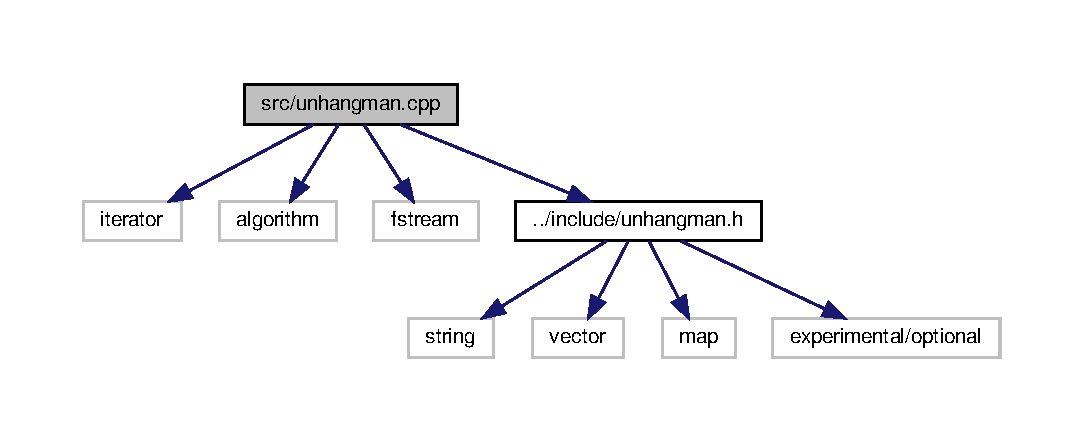
\includegraphics[width=350pt]{unhangman_8cpp__incl}
\end{center}
\end{figure}
\subsection*{Functions}
\begin{DoxyCompactItemize}
\item 
std\+::vector$<$ std\+::string $>$ \hyperlink{unhangman_8cpp_ada47e9338f9e87b423f8214dc4a736e6}{read\+\_\+dictionary} (const std\+::string \&path)
\begin{DoxyCompactList}\small\item\em Fill a vector of strings from a file. \end{DoxyCompactList}\item 
std\+::vector$<$ std\+::string $>$ \hyperlink{unhangman_8cpp_a4905d4615c76e8b03b2485034f1dbda1}{filter\+\_\+length} (const std\+::vector$<$ std\+::string $>$ \&dictionary, unsigned length)
\begin{DoxyCompactList}\small\item\em Filters out words that don\textquotesingle{}t match the desired length. \end{DoxyCompactList}\item 
std\+::vector$<$ std\+::string $>$ \hyperlink{unhangman_8cpp_ad47d17ecfd4f083c423979fec14e17f7}{filter\+\_\+pattern} (const std\+::vector$<$ std\+::string $>$ \&dictionary, const std\+::string \&pattern, char wildcard)
\begin{DoxyCompactList}\small\item\em Filter words that dont match the provided pattern. \end{DoxyCompactList}\item 
std\+::map$<$ char, unsigned $>$ \hyperlink{unhangman_8cpp_a5e092642187020491952150cd43d0ee1}{count\+\_\+character\+\_\+frequency} (const std\+::vector$<$ std\+::string $>$ \&dictionary, const std\+::string \&pattern)
\begin{DoxyCompactList}\small\item\em Counts the appearance of characters in words. Each character is counted once per word. If it\textquotesingle{}s possition matches the pattern\textquotesingle{}s, it\textquotesingle{}s ignored. \end{DoxyCompactList}\item 
std\+::vector$<$ char $>$ \hyperlink{unhangman_8cpp_a3663781c1785f8bd725da940b07e2fb9}{frequency\+\_\+to\+\_\+array} (const std\+::map$<$ char, unsigned $>$ \&character\+\_\+frequency)
\begin{DoxyCompactList}\small\item\em Transforms a map of characters and their appearance counters to an array sorted by the appearance counter. \end{DoxyCompactList}\item 
std\+::experimental\+::optional$<$ char $>$ \hyperlink{unhangman_8cpp_a8df83002e03d77a8976c05beab222dd4}{get\+\_\+next\+\_\+char} (const std\+::vector$<$ char $>$ \&char\+\_\+array, const std\+::string \&ignore)
\begin{DoxyCompactList}\small\item\em Get the character that apeared in the most words. \end{DoxyCompactList}\item 
std\+::experimental\+::optional$<$ char $>$ \hyperlink{unhangman_8cpp_a7e06b1d46a5289a2738001193cccb5a2}{get\+\_\+next\+\_\+vowel} (const std\+::vector$<$ char $>$ \&char\+\_\+array, const std\+::string \&ignore)
\begin{DoxyCompactList}\small\item\em Get the vowel that apeared in the most words. \end{DoxyCompactList}\item 
std\+::experimental\+::optional$<$ char $>$ \hyperlink{unhangman_8cpp_aab30499b410710eeeeb7688234ee5aef}{get\+\_\+next\+\_\+constant} (const std\+::vector$<$ char $>$ \&char\+\_\+array, const std\+::string \&ignore)
\begin{DoxyCompactList}\small\item\em Get the constatnt that apeared in the most words. \end{DoxyCompactList}\item 
std\+::experimental\+::optional$<$ std\+::vector$<$ unsigned $>$ $>$ \hyperlink{unhangman_8cpp_a8b79ef16e04c4f46d2204a618a3b6fb9}{find\+\_\+char\+\_\+positions} (const std\+::vector$<$ std\+::string $>$ \&dictionary, char c)
\begin{DoxyCompactList}\small\item\em If a character appears in the same possitions in all provided words, it returns their positions. \end{DoxyCompactList}\item 
std\+::string \hyperlink{unhangman_8cpp_adbfbe949254445d2547b52546f56c07f}{remove\+\_\+pattern} (const std\+::string \&word, const std\+::string \&pattern, char wildcard)
\begin{DoxyCompactList}\small\item\em Removes the characters of pattern from word. \end{DoxyCompactList}\item 
std\+::vector$<$ std\+::string $>$ \hyperlink{unhangman_8cpp_ab27e44b6f131bd9d905bfeaad5c077c6}{must\+\_\+contain} (const std\+::vector$<$ std\+::string $>$ \&dictionary, char c, const std\+::string \&pattern)
\begin{DoxyCompactList}\small\item\em Returns a vector of words that contain the specified character, ignoring it\textquotesingle{}s appearence in the pattern (if provided) \end{DoxyCompactList}\item 
std\+::vector$<$ std\+::string $>$ \hyperlink{unhangman_8cpp_a704e6e379a70c218fc80e3cea533d634}{must\+\_\+not\+\_\+contain} (const std\+::vector$<$ std\+::string $>$ \&dictionary, char c, const std\+::string \&pattern)
\begin{DoxyCompactList}\small\item\em Returns a vector of words that don\textquotesingle{}t contain the specified character, ignoring it\textquotesingle{}s appearence in the pattern (if provided) \end{DoxyCompactList}\end{DoxyCompactItemize}


\subsection{Detailed Description}
Implementations of all the functions. 



\subsection{Function Documentation}
\mbox{\Hypertarget{unhangman_8cpp_a5e092642187020491952150cd43d0ee1}\label{unhangman_8cpp_a5e092642187020491952150cd43d0ee1}} 
\index{unhangman.\+cpp@{unhangman.\+cpp}!count\+\_\+character\+\_\+frequency@{count\+\_\+character\+\_\+frequency}}
\index{count\+\_\+character\+\_\+frequency@{count\+\_\+character\+\_\+frequency}!unhangman.\+cpp@{unhangman.\+cpp}}
\subsubsection{\texorpdfstring{count\+\_\+character\+\_\+frequency()}{count\_character\_frequency()}}
{\footnotesize\ttfamily std\+::map$<$char, unsigned$>$ count\+\_\+character\+\_\+frequency (\begin{DoxyParamCaption}\item[{const std\+::vector$<$ std\+::string $>$ \&}]{dictionary,  }\item[{const std\+::string \&}]{pattern = {\ttfamily \char`\"{}\char`\"{}} }\end{DoxyParamCaption})}



Counts the appearance of characters in words. Each character is counted once per word. If it\textquotesingle{}s possition matches the pattern\textquotesingle{}s, it\textquotesingle{}s ignored. 


\begin{DoxyParams}{Parameters}
{\em dictionary} & The words to check \\
\hline
{\em pattern} & The pattern to ignore\\
\hline
\end{DoxyParams}
\begin{DoxyReturn}{Returns}
A map of characters and their appearance counters 
\end{DoxyReturn}
\mbox{\Hypertarget{unhangman_8cpp_a4905d4615c76e8b03b2485034f1dbda1}\label{unhangman_8cpp_a4905d4615c76e8b03b2485034f1dbda1}} 
\index{unhangman.\+cpp@{unhangman.\+cpp}!filter\+\_\+length@{filter\+\_\+length}}
\index{filter\+\_\+length@{filter\+\_\+length}!unhangman.\+cpp@{unhangman.\+cpp}}
\subsubsection{\texorpdfstring{filter\+\_\+length()}{filter\_length()}}
{\footnotesize\ttfamily std\+::vector$<$std\+::string$>$ filter\+\_\+length (\begin{DoxyParamCaption}\item[{const std\+::vector$<$ std\+::string $>$ \&}]{dictionary,  }\item[{unsigned}]{length }\end{DoxyParamCaption})}



Filters out words that don\textquotesingle{}t match the desired length. 


\begin{DoxyParams}{Parameters}
{\em dictionary} & The words to check \\
\hline
{\em length} & The required length\\
\hline
\end{DoxyParams}
\begin{DoxyReturn}{Returns}
A vector$<$string$>$ of words that match the length 
\end{DoxyReturn}
\mbox{\Hypertarget{unhangman_8cpp_ad47d17ecfd4f083c423979fec14e17f7}\label{unhangman_8cpp_ad47d17ecfd4f083c423979fec14e17f7}} 
\index{unhangman.\+cpp@{unhangman.\+cpp}!filter\+\_\+pattern@{filter\+\_\+pattern}}
\index{filter\+\_\+pattern@{filter\+\_\+pattern}!unhangman.\+cpp@{unhangman.\+cpp}}
\subsubsection{\texorpdfstring{filter\+\_\+pattern()}{filter\_pattern()}}
{\footnotesize\ttfamily std\+::vector$<$std\+::string$>$ filter\+\_\+pattern (\begin{DoxyParamCaption}\item[{const std\+::vector$<$ std\+::string $>$ \&}]{dictionary,  }\item[{const std\+::string \&}]{pattern,  }\item[{char}]{wildcard = {\ttfamily \textquotesingle{}~$\ast$\textquotesingle{}} }\end{DoxyParamCaption})}



Filter words that dont match the provided pattern. 


\begin{DoxyParams}{Parameters}
{\em dictionary} & The words to check \\
\hline
{\em pattern} & A string to match all words. E.\+g. \char`\"{}pot$\ast$to\char`\"{} \\
\hline
{\em wildcard} & The character to ignore in the pattern. Default \textquotesingle{}$\ast$\textquotesingle{}\\
\hline
\end{DoxyParams}
\begin{DoxyReturn}{Returns}
A vector$<$string$>$ of words that match the pattern 
\end{DoxyReturn}
\mbox{\Hypertarget{unhangman_8cpp_a8b79ef16e04c4f46d2204a618a3b6fb9}\label{unhangman_8cpp_a8b79ef16e04c4f46d2204a618a3b6fb9}} 
\index{unhangman.\+cpp@{unhangman.\+cpp}!find\+\_\+char\+\_\+positions@{find\+\_\+char\+\_\+positions}}
\index{find\+\_\+char\+\_\+positions@{find\+\_\+char\+\_\+positions}!unhangman.\+cpp@{unhangman.\+cpp}}
\subsubsection{\texorpdfstring{find\+\_\+char\+\_\+positions()}{find\_char\_positions()}}
{\footnotesize\ttfamily std\+::experimental\+::optional$<$std\+::vector$<$unsigned$>$ $>$ find\+\_\+char\+\_\+positions (\begin{DoxyParamCaption}\item[{const std\+::vector$<$ std\+::string $>$ \&}]{dictionary,  }\item[{char}]{c }\end{DoxyParamCaption})}



If a character appears in the same possitions in all provided words, it returns their positions. 


\begin{DoxyParams}{Parameters}
{\em dictionary} & The words to check \\
\hline
{\em c} & The character to find positions\\
\hline
\end{DoxyParams}
\begin{DoxyReturn}{Returns}
A vector$<$unsigned$>$ with the positions of the character 
\end{DoxyReturn}
\mbox{\Hypertarget{unhangman_8cpp_a3663781c1785f8bd725da940b07e2fb9}\label{unhangman_8cpp_a3663781c1785f8bd725da940b07e2fb9}} 
\index{unhangman.\+cpp@{unhangman.\+cpp}!frequency\+\_\+to\+\_\+array@{frequency\+\_\+to\+\_\+array}}
\index{frequency\+\_\+to\+\_\+array@{frequency\+\_\+to\+\_\+array}!unhangman.\+cpp@{unhangman.\+cpp}}
\subsubsection{\texorpdfstring{frequency\+\_\+to\+\_\+array()}{frequency\_to\_array()}}
{\footnotesize\ttfamily std\+::vector$<$char$>$ frequency\+\_\+to\+\_\+array (\begin{DoxyParamCaption}\item[{const std\+::map$<$ char, unsigned $>$ \&}]{character\+\_\+frequency }\end{DoxyParamCaption})}



Transforms a map of characters and their appearance counters to an array sorted by the appearance counter. 


\begin{DoxyParams}{Parameters}
{\em character\+\_\+frequency} & A map of characters and their appearance counters\\
\hline
\end{DoxyParams}
\begin{DoxyReturn}{Returns}
An array sorted by the appearance counter 
\end{DoxyReturn}
\mbox{\Hypertarget{unhangman_8cpp_a8df83002e03d77a8976c05beab222dd4}\label{unhangman_8cpp_a8df83002e03d77a8976c05beab222dd4}} 
\index{unhangman.\+cpp@{unhangman.\+cpp}!get\+\_\+next\+\_\+char@{get\+\_\+next\+\_\+char}}
\index{get\+\_\+next\+\_\+char@{get\+\_\+next\+\_\+char}!unhangman.\+cpp@{unhangman.\+cpp}}
\subsubsection{\texorpdfstring{get\+\_\+next\+\_\+char()}{get\_next\_char()}}
{\footnotesize\ttfamily std\+::experimental\+::optional$<$char$>$ get\+\_\+next\+\_\+char (\begin{DoxyParamCaption}\item[{const std\+::vector$<$ char $>$ \&}]{char\+\_\+array,  }\item[{const std\+::string \&}]{ignore = {\ttfamily \char`\"{}\char`\"{}} }\end{DoxyParamCaption})}



Get the character that apeared in the most words. 


\begin{DoxyParams}{Parameters}
{\em char\+\_\+array} & Characters sorted by appearance frequency \\
\hline
{\em ignore} & Characters to ignore if they come up\\
\hline
\end{DoxyParams}
\begin{DoxyReturn}{Returns}
The next possible character. if there are none returns nullopt 
\end{DoxyReturn}
\mbox{\Hypertarget{unhangman_8cpp_aab30499b410710eeeeb7688234ee5aef}\label{unhangman_8cpp_aab30499b410710eeeeb7688234ee5aef}} 
\index{unhangman.\+cpp@{unhangman.\+cpp}!get\+\_\+next\+\_\+constant@{get\+\_\+next\+\_\+constant}}
\index{get\+\_\+next\+\_\+constant@{get\+\_\+next\+\_\+constant}!unhangman.\+cpp@{unhangman.\+cpp}}
\subsubsection{\texorpdfstring{get\+\_\+next\+\_\+constant()}{get\_next\_constant()}}
{\footnotesize\ttfamily std\+::experimental\+::optional$<$char$>$ get\+\_\+next\+\_\+constant (\begin{DoxyParamCaption}\item[{const std\+::vector$<$ char $>$ \&}]{char\+\_\+array,  }\item[{const std\+::string \&}]{ignore = {\ttfamily \char`\"{}\char`\"{}} }\end{DoxyParamCaption})}



Get the constatnt that apeared in the most words. 


\begin{DoxyParams}{Parameters}
{\em char\+\_\+array} & Characters sorted by appearance frequency \\
\hline
{\em ignore} & Characters to ignore if they come up\\
\hline
\end{DoxyParams}
\begin{DoxyReturn}{Returns}
The next possible constant character. if there are none returns nullopt 
\end{DoxyReturn}
\mbox{\Hypertarget{unhangman_8cpp_a7e06b1d46a5289a2738001193cccb5a2}\label{unhangman_8cpp_a7e06b1d46a5289a2738001193cccb5a2}} 
\index{unhangman.\+cpp@{unhangman.\+cpp}!get\+\_\+next\+\_\+vowel@{get\+\_\+next\+\_\+vowel}}
\index{get\+\_\+next\+\_\+vowel@{get\+\_\+next\+\_\+vowel}!unhangman.\+cpp@{unhangman.\+cpp}}
\subsubsection{\texorpdfstring{get\+\_\+next\+\_\+vowel()}{get\_next\_vowel()}}
{\footnotesize\ttfamily std\+::experimental\+::optional$<$char$>$ get\+\_\+next\+\_\+vowel (\begin{DoxyParamCaption}\item[{const std\+::vector$<$ char $>$ \&}]{char\+\_\+array,  }\item[{const std\+::string \&}]{ignore = {\ttfamily \char`\"{}\char`\"{}} }\end{DoxyParamCaption})}



Get the vowel that apeared in the most words. 


\begin{DoxyParams}{Parameters}
{\em char\+\_\+array} & Characters sorted by appearance frequency \\
\hline
{\em ignore} & Characters to ignore if they come up\\
\hline
\end{DoxyParams}
\begin{DoxyReturn}{Returns}
The next possible vowel character. if there are none returns nullopt 
\end{DoxyReturn}
\mbox{\Hypertarget{unhangman_8cpp_ab27e44b6f131bd9d905bfeaad5c077c6}\label{unhangman_8cpp_ab27e44b6f131bd9d905bfeaad5c077c6}} 
\index{unhangman.\+cpp@{unhangman.\+cpp}!must\+\_\+contain@{must\+\_\+contain}}
\index{must\+\_\+contain@{must\+\_\+contain}!unhangman.\+cpp@{unhangman.\+cpp}}
\subsubsection{\texorpdfstring{must\+\_\+contain()}{must\_contain()}}
{\footnotesize\ttfamily std\+::vector$<$std\+::string$>$ must\+\_\+contain (\begin{DoxyParamCaption}\item[{const std\+::vector$<$ std\+::string $>$ \&}]{dictionary,  }\item[{char}]{c,  }\item[{const std\+::string \&}]{pattern = {\ttfamily \char`\"{}\char`\"{}} }\end{DoxyParamCaption})}



Returns a vector of words that contain the specified character, ignoring it\textquotesingle{}s appearence in the pattern (if provided) 


\begin{DoxyParams}{Parameters}
{\em dictionary} & A vector of words that you are currently choosing from \\
\hline
{\em c} & The character that the words must contain \\
\hline
{\em pattern} & The pattern wich should be ignored in all words\\
\hline
\end{DoxyParams}
\begin{DoxyReturn}{Returns}
a vector of words that contain the specified character. 
\end{DoxyReturn}
\mbox{\Hypertarget{unhangman_8cpp_a704e6e379a70c218fc80e3cea533d634}\label{unhangman_8cpp_a704e6e379a70c218fc80e3cea533d634}} 
\index{unhangman.\+cpp@{unhangman.\+cpp}!must\+\_\+not\+\_\+contain@{must\+\_\+not\+\_\+contain}}
\index{must\+\_\+not\+\_\+contain@{must\+\_\+not\+\_\+contain}!unhangman.\+cpp@{unhangman.\+cpp}}
\subsubsection{\texorpdfstring{must\+\_\+not\+\_\+contain()}{must\_not\_contain()}}
{\footnotesize\ttfamily std\+::vector$<$std\+::string$>$ must\+\_\+not\+\_\+contain (\begin{DoxyParamCaption}\item[{const std\+::vector$<$ std\+::string $>$ \&}]{dictionary,  }\item[{char}]{c,  }\item[{const std\+::string \&}]{pattern = {\ttfamily \char`\"{}\char`\"{}} }\end{DoxyParamCaption})}



Returns a vector of words that don\textquotesingle{}t contain the specified character, ignoring it\textquotesingle{}s appearence in the pattern (if provided) 


\begin{DoxyParams}{Parameters}
{\em dictionary} & A vector of words that you are currently choosing from \\
\hline
{\em c} & The character that the words must not contain \\
\hline
{\em pattern} & The pattern wich should be ignored in all words\\
\hline
\end{DoxyParams}
\begin{DoxyReturn}{Returns}
a vector of words that don\textquotesingle{}t contain the specified character. 
\end{DoxyReturn}
\mbox{\Hypertarget{unhangman_8cpp_ada47e9338f9e87b423f8214dc4a736e6}\label{unhangman_8cpp_ada47e9338f9e87b423f8214dc4a736e6}} 
\index{unhangman.\+cpp@{unhangman.\+cpp}!read\+\_\+dictionary@{read\+\_\+dictionary}}
\index{read\+\_\+dictionary@{read\+\_\+dictionary}!unhangman.\+cpp@{unhangman.\+cpp}}
\subsubsection{\texorpdfstring{read\+\_\+dictionary()}{read\_dictionary()}}
{\footnotesize\ttfamily std\+::vector$<$std\+::string$>$ read\+\_\+dictionary (\begin{DoxyParamCaption}\item[{const std\+::string \&}]{path }\end{DoxyParamCaption})}



Fill a vector of strings from a file. 


\begin{DoxyParams}{Parameters}
{\em path} & Where to find the dictinary\\
\hline
\end{DoxyParams}
\begin{DoxyReturn}{Returns}
vector$<$string$>$ containing lines of the dictionary 
\end{DoxyReturn}
\mbox{\Hypertarget{unhangman_8cpp_adbfbe949254445d2547b52546f56c07f}\label{unhangman_8cpp_adbfbe949254445d2547b52546f56c07f}} 
\index{unhangman.\+cpp@{unhangman.\+cpp}!remove\+\_\+pattern@{remove\+\_\+pattern}}
\index{remove\+\_\+pattern@{remove\+\_\+pattern}!unhangman.\+cpp@{unhangman.\+cpp}}
\subsubsection{\texorpdfstring{remove\+\_\+pattern()}{remove\_pattern()}}
{\footnotesize\ttfamily std\+::string remove\+\_\+pattern (\begin{DoxyParamCaption}\item[{const std\+::string \&}]{word,  }\item[{const std\+::string \&}]{pattern,  }\item[{char}]{wildcard = {\ttfamily \textquotesingle{}~$\ast$\textquotesingle{}} }\end{DoxyParamCaption})}



Removes the characters of pattern from word. 


\begin{DoxyParams}{Parameters}
{\em word} & The word you need to clean up \\
\hline
{\em pattern} & The characters you want removed from word \\
\hline
{\em wildcard} & If this character is in the pattern it will not be removed from word\\
\hline
\end{DoxyParams}
\begin{DoxyReturn}{Returns}
The word but without any characters of the pattern 
\end{DoxyReturn}

%--- End generated contents ---

% Index
\backmatter
\newpage
\phantomsection
\clearemptydoublepage
\addcontentsline{toc}{chapter}{Index}
\printindex

\end{document}
